\documentclass{IEEEtran}
\interdisplaylinepenalty=2500

\usepackage{tikz}
\usetikzlibrary{arrows.meta}
\usepackage{iftex}
\ifXeTeX
  \usepackage{fontspec}
\else\ifLuaTeX
  \usepackage{fontspec}
\else
  \usepackage[utf8]{inputenc}
  \usepackage[T5]{fontenc}
  \usepackage[vietnamese]{babel}
\fi\fi

\usepackage{amsmath,amssymb,amsfonts}
\allowdisplaybreaks
\newcommand{\R}{\mathbb{R}}
\usepackage{pifont}
\DeclareRobustCommand{\cmark}{\ding{51}}
\DeclareRobustCommand{\xmark}{\ding{55}}
\usepackage{float}
\usepackage{tikz}
\usetikzlibrary{arrows.meta,positioning,calc}
\usepackage{booktabs}
\usepackage[caption=false,font=footnotesize]{subfig}
\usepackage{caption}
\captionsetup{justification=centering}

\usepackage{siunitx}
\sisetup{
  table-number-alignment = center,
  round-mode = places,
  round-precision = 2,
  scientific-notation = true
}

% Reduce excess vertical space around floats
\setlength{\floatsep}{4pt plus 1pt minus 1pt}
\setlength{\textfloatsep}{6pt plus 1pt minus 1pt}
\setlength{\intextsep}{4pt plus 1pt minus 1pt}
\setlength{\dbltextfloatsep}{6pt plus 1pt minus 1pt}
\setlength{\dblfloatsep}{4pt plus 1pt minus 1pt}

\title{SphyL-Vessel: Ràng buộc vật lý lồi--trơn cho dự báo quỹ đạo tàu từ dữ liệu AIS}

\author{
  Nhữ Phạm Quang Mạnh\\
  Nghiên cứu độc lập\\
  TP. Hồ Chí Minh, Việt Nam\\
  \texttt{py.quangmanh.ai@gmail.com}
}
\raggedbottom
\begin{document}

% ============================================================
% SECTION III — PHƯƠNG PHÁP VÀ ĐỀ XUẤT
% ============================================================
\section{PHƯƠNG PHÁP VÀ ĐỀ XUẤT}

% ============================================================
% 3.1  Tổng quan phương pháp
% ============================================================
\subsection{Tổng quan phương pháp}\label{sec:overview}

Mục tiêu chính của nghiên cứu này là dự báo quỹ đạo tàu một bước
($t_{10}$) từ cửa sổ 10 bước quan sát quá khứ ($t_0 \ldots t_9$),
đồng thời đảm bảo rằng vị trí dự báo luôn nằm trong miền chuyển động
khả thi về mặt vật lý.

\textbf{Bài toán gốc.}
Cho chuỗi quan sát $\{\mathbf{x}_{t_0}, \mathbf{x}_{t_1},\ldots,\mathbf{x}_{t_9}\}$
gồm 10 bước với 9 đặc trưng mỗi bước
(SOG, sin/cos Heading, sin/cos COG, $X_\text{norm}$, $Y_\text{norm}$, sin/cos giờ),
mục tiêu là dự báo vị trí tàu tại bước $t_{10}$:
\[
\hat{\mathbf{p}}_{10} = f_\theta(\mathbf{X}_{t_0:t_9}),
\quad \mathbf{X} \in \mathbb{R}^{10\times 9},
\quad \hat{\mathbf{p}}_{10} \in \mathbb{R}^2.
\]
Hàm $f_\theta$ là backbone LSTM với attention pooling
(không đổi giữa Baseline và SphyL--Vessel).
Điểm khác biệt duy nhất nằm ở \textbf{hàm loss huấn luyện}:
SphyL--Vessel bổ sung một loss vật lý lồi--trơn vào MSE gốc.

\textbf{Tính chất architecture-invariant.}
Thiết kế của SphyL--Vessel là \textbf{không phụ thuộc kiến trúc}
(\textit{architecture-invariant}): lớp loss Tube--Stomach
có thể gắn vào bất kỳ backbone nào xuất ra tọa độ $(x, y)$
--- LSTM, GRU, Transformer, hay mô hình đồ thị ---
mà không cần thay đổi cấu trúc mạng. Overhead duy nhất là tính
khoảng cách hình học và softplus trong forward pass của loss.

\textbf{Ý tưởng tổng quát.}
Các phương pháp học sâu thuần (LSTM, GRU, Transformer) tối ưu hóa
chủ yếu thông qua hàm MSE, do đó chúng chỉ học mối quan hệ thống kê
trong dữ liệu huấn luyện mà không có bất kỳ ràng buộc nào về tính
khả dĩ vật lý của kết quả dự đoán.
Hệ quả là khi tàu đổi hướng đột ngột hoặc chuyển động trong vùng hẹp
(gần bờ, gần cảng), sai số dự báo có thể lớn và không an toàn.

SphyL--Vessel (\textbf{Sph}erical \textbf{y}ielding
\textbf{L}oss for \textbf{Vessel}) đề xuất bổ sung một
\textbf{lớp ràng buộc hình học lồi--trơn} vào hàm loss gốc.
Cụ thể, tại mỗi bước dự báo, một \textbf{hành lang hình học}
(\textit{tube}) được xây dựng dựa trên vận tốc và hướng hiện tại của tàu;
mọi điểm nằm ngoài hành lang này sẽ bị phạt tỷ lệ với khoảng cách
tới biên hành lang. Kết hợp với hàm \textbf{Stomach} (dạng Beta-shape
bất đối xứng) giúp phân bổ phạt trơn hơn so với phạt hard-threshold.

\textbf{Flow diagram tổng quan} của phương pháp được trình bày
trong Hình~\ref{fig:method-overview}.

% ===== FIGURE 1 =====
\begin{figure}[H]
\centering
\begin{tikzpicture}[
  nd/.style={draw, rounded corners=2pt, minimum height=0.7cm,
             minimum width=2.4cm, font=\scriptsize\sffamily,
             align=center, fill=white},
  ar/.style={-{Stealth[length=1.5mm]}, thin},
  node distance=0.5cm
]
  \node[nd] (inp)  {AIS input\\$t_0\!\ldots\!t_9$ · 9 features};
  \node[nd, below=of inp]  (pre) {Preprocess\\Filter · normalize};
  \node[nd, below=of pre]  (mdl) {LSTM + attention\\hidden=256 · 2 layers};
  \node[nd, below left =0.6cm and -0.5cm of mdl] (pred)
    {Predicted $\hat{\mathbf{p}}_{10}$\\$\mathcal{L}_{\text{MSE}}=\|\hat{p}-y^*\|^2$};
  \node[nd, below right=0.6cm and -0.5cm of mdl] (tube)
    {Build tube\\Ellipsoid + Beta-shape};
  \node[nd, minimum width=3.4cm, below=1.6cm of mdl] (loss)
    {$\mathcal{L}_{\text{MSE}}+\lambda(t)\cdot\mathcal{L}_{\text{tube}}$\\
     $\lambda$ ramp 15 ep · $\lambda_{\max}=0.003$};
  \node[nd, below=of loss] (upd)
    {Update $\theta$ · Backprop · AdamW};

  \draw[ar] (inp)--(pre);
  \draw[ar] (pre)--(mdl);
  \draw[ar] (mdl)--(pred);
  \draw[ar] (mdl)--(tube);
  \draw[ar] (pred)--(loss);
  \draw[ar] (tube)--(loss);
  \draw[ar] (loss)--(upd);
\end{tikzpicture}
\caption{Tổng quan phương pháp SphyL--Vessel.}
\label{fig:method-overview}
\end{figure}

\textbf{Các đóng góp chính của chương này:}
\begin{enumerate}
  \item Xây dựng hành lang vật lý \textbf{lồi--trơn} dựa trên ràng buộc
        tốc độ và hướng chuyển động, biểu diễn bằng tổ hợp elip ngoài
        và bụng Beta-shape bất đối xứng bên trong.
  \item Thiết kế hàm loss bổ sung Tube--Stomach với kỹ thuật
        \textbf{soft penalty} (thay vì hard threshold), khả vi toàn cục,
        không ảnh hưởng quá trình tối ưu hóa MSE gốc.
  \item Phân tích sự khác biệt giữa SphyL, PINN và TPK trên bình diện
        đảm bảo ràng buộc vật lý.
\end{enumerate}

% ============================================================
% 3.2  Bộ ký hiệu và đại lượng vật lý
%      (chuyển từ Mục II cũ)
% ============================================================
\subsection{Bộ ký hiệu và đại lượng vật lý}\label{sec:notation}

\begin{table}[H]
\caption{Các ký hiệu chính trong \emph{SphyL--Vessel}.}
\label{tab:sphyl-symbols}
\centering
\begin{tabular}{ll}
\hline
Ký hiệu & Diễn giải \\
\hline\\[4pt]
$p_0=(x_0,y_0)$ & Vị trí ban đầu trong hệ toàn cục \\
$\hat{p}=(x,y)$ & Vị trí dự đoán sau khoảng $\Delta t$ \\
$v_0$ & Vận tốc tại $t_0$ \\
$\theta_0$ & Góc heading ban đầu so với trục $Ox$ \\
$d=\theta_{\text{motion}}-\theta_0$ & Chênh lệch hướng chuyển động và heading \\
$\Delta t$ & Độ dài bước dự báo \\
$a_t^{\max}$ & Gia tốc cực đại dọc (thúc--phanh) \\
$a_n^{\max}$ & Gia tốc cực đại ngang (rẽ) \\
$v_{\max}$ & Vận tốc cực đại \\
$e_{\parallel},e_{\perp}$ & Cơ sở trực chuẩn cục bộ (song song/vuông góc) \\
$\Delta p=\hat{p}-p_0$ & Vectơ dịch chuyển \\
$s=\Delta p \cdot e_{\parallel}$ & Tiến dọc \\
$y=\Delta p \cdot e_{\perp}$ & Lệch ngang \\
$a,b$ & Bán trục dọc/ngang của elip \\
$M$ & Ma trận xác định dương trong quadratic form \\
$\tau$ & Tham số kích hoạt mềm (turn-rate/gia tốc) \\
$r_{\text{base}}, B_{\max}, s_{\max}$ & Tham số hành lang tube \\
$\rho(s)$ & Hàm bụng chuẩn $4t(1-t)$ \\
$\rho_{\alpha,\beta}(t)$ & Hàm bụng cải tiến Beta-shape \\
$p_c(s)$ & Đường centerline cong \\
$s_{\text{cap}}$ & Giới hạn động (forward cap) \\
$\phi_{\text{lat}},\phi_{\text{fwd}},\phi_{\text{prog}}$ & Phạt loss ngang/dọc/tiến \\
$\lambda, \alpha_m$ & Hệ số loss vật lý / pha trộn dữ liệu \\
$\phi_{\kappa}(u)$ & Softplus: $\tfrac{1}{\kappa}\log(1+e^{\kappa u})$ \\
\\[4pt]
\hline
\end{tabular}
\end{table}

% ============================================================
% 3.3  Khung tọa độ cục bộ + centerline cong
%      (chuyển từ Mục II cũ)
% ============================================================
\subsection{Khung tọa độ cục bộ và centerline cong}\label{sec:local-frame}

Từ trạng thái ban đầu, thiết lập hệ trục:
\[
e_{\parallel} = R(d)\,e_{\text{head}},
\qquad
e_{\perp} = (-e_{\parallel,y},\,e_{\parallel,x}),
\]
trong đó $R(d)$ là phép quay một góc $d$.
Mọi dự đoán $\hat{p}$ được quy chiếu về tọa độ cục bộ:
\[
s=(\hat{p}-p_0)\cdot e_{\parallel},
\qquad
y=(\hat{p}-p_0)\cdot e_{\perp}.
\]

\textbf{Centerline cong.}
Trong phiên bản cải tiến, thay vì giữ trục $e_{\parallel}$ cố định,
chúng tôi định nghĩa đường trung tâm cong:
\[
p_c(s) = p_0 + s e_{\parallel} + \delta(s)\,e_{\perp},
\qquad \delta(s) = \alpha_{\text{curve}}\,s(1-s),
\]
cho phép khung tọa độ $(s,y)$ uốn theo hướng chuyển động,
phản ánh động học tốt hơn khi tàu cua hoặc đổi hướng.

% ============================================================
% 3.4  Miền elip cứng → elip dịch tâm → siêu elip
%      (chuyển từ Mục II cũ)
% ============================================================
\subsection{Miền khả đạt: từ elip cứng đến siêu elip}\label{sec:ellipse}

\subsubsection{Miền elip cứng: khởi nguyên lý thuyết}
Trong bước thời gian $\Delta t$, quỹ đạo khả đạt giới hạn bởi:
\begin{IEEEeqnarray}{rCl}
0 \le s &\le& v_0 \Delta t + \tfrac12 a_t^{\max}\,\Delta t^{2},\\
|y|     &\le& \tfrac12 a_n^{\max}\,\Delta t^{2},\\
v_0     &\le& v_{\max}.
\end{IEEEeqnarray}
Hình học hóa: mô hình miền khả đạt là elip centered tại $p_0$, với bán trục
\[
a = v_0 \Delta t + \tfrac{1}{2} a_t^{\max} (\Delta t)^2,
\qquad
b = \tfrac{1}{2} a_n^{\max} (\Delta t)^2.
\]
Điều kiện khả thi:
\[
\mathcal{E} = \{(s,y) \;\mid\; \tfrac{s^2}{a^2} + \tfrac{y^2}{b^2} \leq 1 \}.
\]

\subsubsection{Elip dịch tâm: bù lệch hình học}
Để khắc phục sự đối xứng cứng nhắc, ta cho phép tâm elip dịch chuyển theo hướng tiến dọc.
Trực giác: khi tàu cua hoặc phanh gắt, vùng khả thi thực tế thường dồn về phía trước
(do quán tính) hoặc lệch sang trong cua. Miền mới:
\[
\mathcal{E}_{\text{shift}} = \Big\{ (s,y) \;\Big|\;
\tfrac{(s-c_s)^2}{a^2} + \tfrac{(y-c_y)^2}{b^2} \leq 1 \Big\}.
\]

\subsubsection{Siêu elip: mở rộng linh hoạt}
Một mở rộng tự nhiên là thay norm $L_2$ bằng $L_p$ với $p>2$,
giúp biên cong phẳng hơn và nội dung bao quát rộng hơn:
\[
\mathcal{E}_{p} = \Big\{ (s,y) \;\Big|\;
\Big(\tfrac{|s|}{a}\Big)^p + \Big(\tfrac{|y|}{b}\Big)^p \leq 1 \Big\}.
\]
Siêu elip vẫn giữ tính lồi (với $p \geq 2$) nhưng giảm hiện tượng ``dẹt'' khi $b$ nhỏ.

% ============================================================
% 3.5  Tube--Stomach Corridor
%      (chuyển từ Mục II cũ)
% ============================================================
\subsection{Tube--Stomach Corridor: hành lang bất đối xứng}\label{sec:tube-stomach}

Khắc phục các hạn chế của elip, hành lang được định nghĩa theo $s$:
\[
0 \leq s \leq s_{\max},
\qquad
-|y_R(s)| \leq y \leq y_L(s).
\]

\textbf{Phiên bản gốc.}
Với $\rho(s)=4t(1-t),\,t=s/s_{\max}$,
biên ngang:
\[
y_L(s) = r_{\text{base}} + \tau \cdot B(s), \qquad
y_R(s) = r_{\text{base}} + \tau \cdot B(s).
\]

\textbf{Phiên bản cải tiến.}
Thay vì dùng $\rho(s)$ cứng nhắc,
chúng tôi áp dụng hàm bụng Beta-shape:
\[
\rho_{\alpha,\beta}(t) =
\frac{t^{\alpha}(1-t)^{\beta}}
     {\left(\tfrac{\alpha}{\alpha+\beta}\right)^{\alpha}
      \left(\tfrac{\beta}{\alpha+\beta}\right)^{\beta}},
\qquad t = s/s_{\max}.
\]
Hàm này cho phép điều chỉnh linh hoạt độ phình,
bao quát tốt hơn khi cua gắt hoặc phanh mạnh.

% ============================================================
% 3.6  Loss lồi–trơn & softplus-hinge
%      (chuyển từ Mục II cũ)
% ============================================================
\subsection{Loss lồi--trơn và cơ chế tối ưu}\label{sec:loss}

Loss tổng quát gồm ba thành phần:
\[
\mathcal{L} = (1-\alpha_m)\,\mathcal{L}_{\text{MSE}}
+ \alpha_m \,\mathcal{L}_{\text{MSE-meters}}
+ \lambda \,\mathcal{L}_{\text{phys}}.
\]

\textbf{Cải tiến cap động và progress anchor.}
Để ngăn dự đoán phi lý:
\[
s_{\text{cap}} = \text{clip}\Big((1+0.3\tau)\,s_{\text{tgt}},\,0.3\,s_{\max},\,1.6\,s_{\max}\Big),
\]
và bổ sung phạt tiến đủ:
\[
\phi_{\text{prog}} = [s_{\text{tgt}}-s_{\text{pred}}]_+^2.
\]

\textbf{Hình thức cuối cùng.}
\[
\mathcal{L}_{\text{phys}} =
w_{\text{lat}}\phi_{\text{lat}} +
w_{\text{fwd}}\phi_{\text{fwd}} +
w_{\text{prog}}\phi_{\text{prog}},
\]
trong đó
\[
\phi_{\text{lat}} = [|y|-y_{\text{bdry}}(s)]_+^2,\quad
\phi_{\text{fwd}} = [s_{\text{pred}}-s_{\text{cap}}]_+^2.
\]
Mọi phạt đều qua softplus $\phi_\kappa(u)$ để duy trì gradient mượt.

% ============================================================
% 3.7  Thảo luận biến thể hình học
%      (chuyển từ Mục II cũ)
% ============================================================
\subsection{Thảo luận các biến thể hình học}\label{sec:geometry-discussion}

\begin{figure}[H]
  \centering
  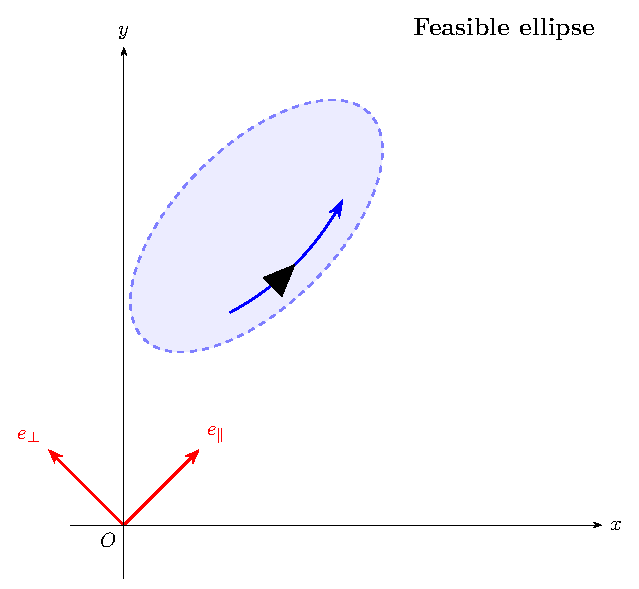
\includegraphics[width=0.85\columnwidth]{tube.pdf}\\[2pt]
  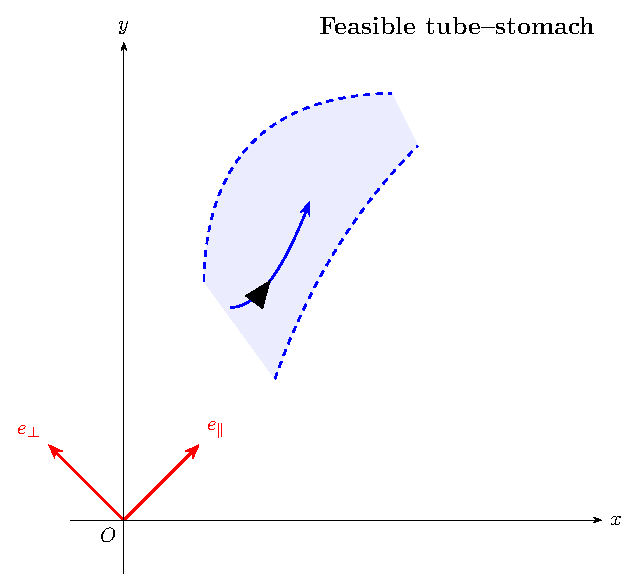
\includegraphics[width=0.85\columnwidth]{tube_3.pdf}
  \caption{So sánh hai dạng vùng khả dĩ: (trên) Feasible ellipse và (dưới) Tube--stomach.}
  \label{fig:ellipse-stomach}
\end{figure}

\textbf{1) Elip cứng.}
Mô hình elip đơn giản, quadratic form gọn gàng, chứng minh tính lồi tức thì.
Đây là \emph{khởi nguyên lý thuyết} của SphyL--Vessel.
Tuy nhiên, với dữ liệu AIS, $b \approx 0$ khiến elip bị dẹt;
chỉ cần nhiễu nhỏ đã rơi ra ngoài, dẫn tới loss cực lớn.
Do đó, elip cứng đẹp về mặt hình học nhưng mong manh trong thực nghiệm.

\textbf{2) Elip dịch tâm.}
Cho phép dịch tâm theo hướng tiến hoặc vào cua để khắc phục phần nào tính đối xứng.
Biến thể này mô tả tốt hơn khi tàu quay hoặc phanh,
nhưng vẫn chỉ là affine transform của elip,
chưa có ``bụng'' để bao quát quán tính trong các tình huống cực trị.

\textbf{3) Siêu elip.}
Với $p>2$, biên cong phẳng hơn, coverage và Hit@100m cải thiện rõ rệt.
Siêu elip vẫn là tập lồi (convex set) và dễ tối ưu,
nhưng chưa có cơ chế động để thích nghi với trạng thái cua hoặc giảm tốc.

\textbf{4) Tube--Stomach.}
Bước nhảy vọt hình học: bất đối xứng tự nhiên, $s_{\max}$ động theo $v_0$,
biên ngang $r_{\text{base}}+B_{\max}\rho(s)$ tạo ``bụng'' mềm để bao quát quán tính khi cua/phanh.
Trong phiên bản cải tiến, hàm $\rho(s)$ được thay bằng $\rho_{\alpha,\beta}(t)$ dạng Beta-shape
và kết hợp với centerline cong, giúp thích nghi tốt hơn với quỹ đạo thực tế.
Tuy nhiên, khác với elip/siêu elip, hình học tube--stomach không còn là tập lồi toàn cục:
đoạn thẳng nối hai điểm trong hành lang có thể chọc ra ngoài ở giữa.
Dù vậy, nhờ thiết kế phạt mềm bằng hinge và softplus,
loss vẫn giữ được đặc tính tối ưu mượt và ổn định,
trở thành lựa chọn thực tế hơn trong huấn luyện.

\medskip
\noindent \textbf{Tóm lại:}
elip cứng đặt nền tảng lý thuyết,
elip dịch tâm và siêu elip mở rộng tính bao phủ,
còn tube--stomach (với bụng linh hoạt và centerline cong)
mang lại giải pháp gần gũi thực tế nhất.
Các biến thể này phản ánh lộ trình tiến hoá từ đơn giản $\to$ thích nghi $\to$ giàu động học.

% ============================================================
% 3.8  Tại sao chọn hình học lồi?
% ============================================================
\subsection{Tại sao chọn hình học lồi?}\label{sec:why-convex}

Một câu hỏi thiết kế quan trọng là: \textit{tại sao miền khả dĩ
vật lý nên được biểu diễn bằng hình học lồi thay vì hình học bất kỳ?}

\subsubsection{Tính chất toán học của tập lồi}
Một tập hợp $\mathcal{C} \subset \R^2$ được gọi là \textbf{lồi}
nếu với mọi $\mathbf{x}, \mathbf{y} \in \mathcal{C}$ và mọi
$\lambda \in [0,1]$, ta có:
\[
\lambda \mathbf{x} + (1-\lambda)\mathbf{y} \in \mathcal{C}.
\]
Điều này có nghĩa là đoạn thẳng nối hai điểm bất kỳ trong $\mathcal{C}$
luôn nằm trọn trong $\mathcal{C}$. Trong bối cảnh quỹ đạo tàu,
tính chất này tương đương với: \textit{nếu cả điểm xuất phát và
điểm đích đều khả dĩ, thì mọi điểm trung gian trên quỹ đạo cũng khả dĩ.}

Đây chính xác là nguyên lý \textbf{quán tính chuyển động} của tàu biển:
khi không có lực bên ngoài đáng kể, tàu không thể "nhảy vọt" qua
một khoảng trống trong không gian --- quỹ đạo liên tục và đoạn thẳng
nối hai vị trí lân cận phải nằm trong miền khả dĩ.

\subsubsection{Khả vi và tối ưu hóa}
Hàm khoảng cách đến một tập lồi (convex distance function)
là \textbf{khả vi gần như mọi nơi} và có gradient Lipschitz.
Điều này cho phép ta xây dựng một penalty term
khả vi trong hàm loss, tránh được hiện tượng gradient vanish/explode
khi điểm dự báo nằm gần biên.

Ngược lại, một miền không lồi (ví dụ: hình sao, miền có lỗ thủng)
sẽ tạo ra các điểm kỳ dị gradient tại các góc lõm,
gây khó khăn cho quá trình tối ưu hóa bằng gradient descent.

\subsubsection{Tốc độ tính toán}
Phép chiếu (projection) lên một tập lồi (convex set) có thể thực hiện
bằng thuật toán \textbf{VFeM} (Vonoroi Facet Expansion Method)
với độ phức tạp tuyến tính theo số biên, trong khi phép chiếu lên
miền không lồi có thể cần tối ưu hóa lặp phức tạp hơn nhiều.
Trong bài toán cần huấn luyện hàng triệu mẫu, yếu tố này là then chốt.

\subsubsection{Tổng hợp}
Bảng~\ref{tab:convex-reason} tổng hợp lý do chọn hình học lồi.

\begin{table}[H]
\centering
\caption{Lý do chọn hình học lồi cho miền khả dĩ vật lý.}
\label{tab:convex-reason}
\begin{tabular}{p{3.0cm}cc}
\toprule
Tiêu chí              & Hình học lồi & Hình học bất kỳ \\
\midrule
Phản ánh quán tính tàu  & \cmark       & \cmark          \\
Khả vi của penalty       & \cmark       & \xmark          \\
Tốc độ tính toán       & Nhanh        & Chậm / kỳ dị   \\
Lipschitz gradient      & \cmark       & \xmark          \\
Đảm bảo miền đóng       & \cmark       & \cmark          \\
\bottomrule
\end{tabular}
\end{table}

% ============================================================
% 3.9  So sánh SphyL với PINN / TPK
% ============================================================
\subsection{So sánh SphyL--Vessel với PINN và TPK}\label{sec:compare-pinn-tpk}

Để định vị rõ đóng góp của SphyL--Vessel, ta so sánh nó với hai
phương pháp ràng buộc vật lý phổ biến: \textbf{PINN}
(Physics-Informed Neural Networks) và \textbf{TPK}
(Trajectory Prediction with Kinematic constraints).

\subsubsection{PINN (Physics-Informed Neural Networks)}
PINN do Raissi et al. (2019) đề xuất, bổ sung các phương trình
vật lý (thường là PDE/ODE) vào hàm loss dưới dạng \textbf{residual}:
\[
\mathcal{L}_{\text{PINN}} = \mathcal{L}_{\text{data}}
  + \lambda_{\text{PDE}} \cdot \mathcal{L}_{\text{PDE}}.
\]
Trong đó $\mathcal{L}_{\text{PDE}} = \frac{1}{N}\sum_i
\left\|\mathcal{F}[\mathbf{u}_\theta(\mathbf{x}_i)]\right\|^2$,
với $\mathcal{F}$ là toán tử vi phân mô phỏng định luật vật lý
(phương trình Navier-Stokes, phương trình động lực học \dots).

\textbf{Hạn chế khi áp dụng cho quỹ đạo tàu:}
\begin{itemize}
  \item Cần mô hình \textbf{giải tích chính xác} của động lực học tàu
        (khối lượng, mô men quán tính, lực cản thủy động \dots).
        Các tham số này \textbf{không có sẵn trong dữ liệu AIS}.
  \item Hàm $\mathcal{L}_{\text{PDE}}$ giả thiết dữ liệu tuân theo
        phương trình vật lý \textit{tại mọi điểm}, nhưng quỹ đạo tàu
        chịu nhiễu đo, thiếu sót và ảnh hưởng bất định (dòng chảy,
        sóng gió cục bộ) --- không thỏa mãn phương trình lý tưởng.
  \item Khó mở rộng (scalability) khi số điểm dữ liệu lớn
        (hàng triệu bản ghi AIS).
\end{itemize}

\subsubsection{TPK (Trajectory Prediction with Kinematic constraints)}
TPK sử dụng ràng buộc động học dưới dạng \textbf{hard constraint}
trong không gian trạng thái mở rộng, ví dụ:
\[
\mathbf{s}_{t+1} = \mathbf{A}\mathbf{s}_t + \mathbf{B}\mathbf{a}_t,
\quad
\mathbf{s}_t = [x_t, y_t, v_x^t, v_y^t]^\top,
\]
với $\mathbf{A}, \mathbf{B}$ là ma trận chuyển đổi cố định theo mô hình
động học (constant velocity hoặc constant acceleration).

\textbf{Hạn chế của TPK:}
\begin{itemize}
  \item Chỉ mô hình hóa mối quan hệ \textbf{tuyến tính} giữa các trạng thái,
        không biểu diễn được \textbf{bất đối xứng} tự nhiên của quỹ đạo tàu
        (bánh lái có thể quay nhanh hơn tàu có thể đổi hướng).
  \item Hard constraint có thể bị vi phạm khi mô hình động lực học
        không chính xác hoặc điều kiện môi trường thay đổi.
  \item Không có cơ chế \textbf{phân bổ penalty theo mật độ} ---
        mọi điểm ngoài miền đều bị phạt như nhau.
\end{itemize}

\subsubsection{Điểm khác biệt cốt lõi của SphyL--Vessel}
SphyL--Vessel lấy cảm hứng từ cả hai nhưng khác biệt ở điểm then chốt:
\begin{itemize}
  \item \textbf{Không cần mô hình vật lý giải tích:}
        hành lang tube được xây dựng \textbf{trực tiếp từ dữ liệu quan sát}
        (SOG, COG) thông qua ràng buộc tốc độ cực đại và profile hình học.
  \item \textbf{Soft penalty lồi-trơn thay vì hard constraint:}
        gradient penalty truyền ngược được toàn cục,
        không bị kẹt tại các điểm biên không khả vi.
  \item \textbf{Beta-shape bất đối xứng (Stomach):}
        cho phép miền phạt "nhọn" phía trước (hướng tàu đang đi)
        và "tròn" phía sau, phản ánh đặc tính điều khiển thực tế của tàu.
  \item \textbf{Ramp-up strategy:}
        tube penalty được tăng dần từ 0, tránh gradient shock và
        cho phép backbone hội tụ ổn định trước khi ràng buộc vật lý
        có hiệu lực.
\end{itemize}

Tổng hợp so sánh ba phương pháp Bảng~\ref{tab:pinn-tpk-comparison}.

\begin{table}[htbp]
\centering
\caption{So sánh SphyL--Vessel với PINN và TPK.}
\label{tab:pinn-tpk-comparison}
\begin{tabular}{p{3.0cm}ccc}
\toprule
Tiêu chí                  & PINN       & TPK        & SphyL--Vessel \\
\midrule
Cần mô hình vật lý giải tích & Có         & Có         & \textbf{Không} \\
Dạng ràng buộc             & Residual   & Hard       & \textbf{Soft penalty} \\
Khả vi toàn cục            & Có         & Không      & \textbf{Có}     \\
Biểu diễn bất đối xứng     & Không      & Không      & \textbf{Có (Beta)} \\
Dữ liệu AIS đủ huấn luyện  & Không      & Không      & \textbf{Có}     \\
Scalability (triệu mẫu)    & Trung bình & Cao        & \textbf{Cao}     \\
Overhead huấn luyện        & Cao (PDE)  & Thấp       & \textbf{Rất thấp} \\
\bottomrule
\end{tabular}
\end{table}

% ============================================================
% 3.10  Luồng nghiệp vụ (Business Flow)
% ============================================================
\subsection{Luồng nghiệp vụ trong hệ thống}\label{sec:business-flow}

Hình~\ref{fig:business-flow} mô tả luồng nghiệp vụ tổng thể
của hệ thống dự báo quỹ đạo tàu dựa trên SphyL--Vessel.

\begin{figure}[H]
\centering
\begin{tikzpicture}[
  nd/.style={draw, rounded corners=2pt, minimum height=0.7cm,
             minimum width=2.6cm, font=\scriptsize\sffamily,
             align=center, fill=white},
  ar/.style={-{Stealth[length=1.5mm]}, thin},
  node distance=0.5cm
]
  \node[nd] (ais)  {AIS data\\NOAA · CA offshore};
  \node[nd, below=of ais]  (proc) {Xử lý dữ liệu\\Lọc SOG · chuẩn hoá};
  \node[nd, below=of proc] (mdl)  {Mô hình dự báo\\LSTM + attn · 800K params};
  \node[nd, below=of mdl]  (phys) {Ràng buộc vật lý\\Tube--Stomach · $\lambda{=}0.003$};
  \node[nd, below=of phys] (out)  {Quỹ đạo dự báo\\$(x,y)$ tại $t_{10}$ · an toàn};

  \draw[ar] (ais)--(proc);
  \draw[ar] (proc)--(mdl);
  \draw[ar] (mdl)--(phys);
  \draw[ar] (phys)--(out);
\end{tikzpicture}
\caption{Luồng nghiệp vụ của hệ thống SphyL--Vessel.}
\label{fig:business-flow}
\end{figure}

\textbf{Mô tả từng bước trong luồng Business Flow:}
\begin{enumerate}
  \item \textbf{AIS Data:} Hệ thống AIS trên tàu phát tín hiệu
        định kỳ (trung bình 60 giây/bản ghi) chứa MMSI, SOG, COG,
        tọa độ (LAT/LON), thời gian. Dữ liệu được thu thập từ
        cơ sở dữ liệu NOAA tại vùng California offshore.
  \item \textbf{Data Processing:} Dữ liệu thô trải qua bước làm sạch
        (lọc tốc độ, lọc thời gian), chuẩn hóa tọa độ (equirectangular
        projection + StandardScaler) và xây dựng cửa sổ 10 bước
        làm đầu vào mô hình.
  \item \textbf{Prediction Model:} Backbone LSTM với attention pooling
        nhận cửa sổ 10 bước, dự báo vị trí tiếp theo.
        Cùng kiến trúc cho cả Baseline và SphyL--Vessel.
  \item \textbf{Physical Constraint Layer (Tube--Stomach):}
        Tại bước huấn luyện, hành lang vật lý được xây dựng từ SOG/COG
        hiện tại; Tube--Stomach loss được cộng vào MSE loss để
        cập nhật gradient. Tại bước suy luận, chỉ có prediction head
        hoạt động, không có overhead ràng buộc.
  \item \textbf{Predicted Trajectory:} Đầu ra là tọa độ $(x,y)$
        tại $t_{10}$, đảm bảo nằm trong miền khả dĩ về vật lý
        (trong hành lang tube), sẵn sàng cho các ứng dụng
        cảnh báo va chạm, quản lý luồng hàng hải.
\end{enumerate}

% ============================================================
% 3.11  Luồng kỹ thuật (Technical Flow)
% ============================================================
\subsection{Luồng kỹ thuật của hệ thống}\label{sec:technical-flow}

Hình~\ref{fig:technical-flow} trình bày chi tiết luồng kỹ thuật từ
dữ liệu đầu vào đến cập nhật trọng số mô hình.

\begin{figure}[H]
\centering
\begin{tikzpicture}[
  nd/.style={draw, rounded corners=2pt, minimum height=0.7cm,
             minimum width=2.6cm, font=\scriptsize\sffamily,
             align=center, fill=white},
  ar/.style={-{Stealth[length=1.5mm]}, thin},
  node distance=0.5cm
]
  \node[nd] (x)
    {$\mathbf{X}\!\in\!\mathbb{R}^{10\times9}$\\10-step · 9 features};
  \node[nd, below=of x] (lstm)
    {Embedding + LSTM$\times$2\\+ attention pooling};
  \node[nd, below=of lstm] (fc)
    {FC(2) $\to\hat{\mathbf{p}}_{10}$ · raw prediction};

  \node[nd, below left =0.6cm and -0.5cm of fc] (lmse)
    {$\mathcal{L}_{\text{MSE}}$\\$\|\hat{p}-y^*\|^2$};
  \node[nd, below right=0.6cm and -0.5cm of fc] (ltube)
    {$\mathcal{L}_{\text{tube}}$\\$\text{softplus}(\text{dist}(\hat{p},\partial\mathcal{T}))$};

  \node[nd, minimum width=3.6cm, below=1.6cm of fc] (loss)
    {$\mathcal{L}_{\text{total}}=\mathcal{L}_{\text{MSE}}+\lambda(t)\cdot\mathcal{L}_{\text{tube}}$\\
     $\lambda$ ramp 15 ep · $\lambda_{\max}=0.003$};
  \node[nd, below=of loss] (bp)
    {Backprop + AdamW · lr=$10^{-4}$};
  \node[nd, below=of bp] (upd)
    {Cập nhật $\theta$ $\to$ epoch mới};

  \draw[ar] (x)--(lstm);
  \draw[ar] (lstm)--(fc);
  \draw[ar] (fc)--(lmse);
  \draw[ar] (fc)--(ltube);
  \draw[ar] (lmse)--(loss);
  \draw[ar] (ltube)--(loss);
  \draw[ar] (loss)--(bp);
  \draw[ar] (bp)--(upd);

  \draw[ar, dashed, -{Stealth[length=1.3mm]}]
    (upd.west) -- ++(-0.6,0) |- (x.west);
  \node[font=\tiny\itshape, left=0.55cm of bp] {vòng lặp};

\end{tikzpicture}
\caption{Luồng kỹ thuật: từ tensor đầu vào đến cập nhật trọng số.}
\label{fig:technical-flow}
\end{figure}

\textbf{Giải thích luồng kỹ thuật:}
\begin{enumerate}
  \item \textbf{Đầu vào} $\mathbf{X} \in \R^{10 \times 9}$: cửa sổ 10 bước
        với 9 đặc trưng (SOG, sin/cos của Heading, sin/cos của COG,
        $X_{\text{norm}}$, $Y_{\text{norm}}$, sin/cos của giờ).
  \item \textbf{Embedding + LSTM $\times$ 2:} Mỗi bước được ánh xạ
        qua embedding layer, qua hai tầng LSTM (hidden=256),
        kết hợp attention pooling để tổng hợp thông tin 10 bước.
  \item \textbf{FC(2) $\rightarrow \hat{\mathbf{p}}_{10}$:}
        Lớp fully-connected đầu ra cho tọa độ $(x,y)$ dự báo tại $t_{10}$.
  \item \textbf{Xây dựng Tube hành lang vật lý:}
        Từ $\hat{\mathbf{p}}_9$ (vị trí cuối cùng quan sát được) và
        SOG, COG hiện tại, xây dựng miền lồi $\mathcal{T}$
        (elip + Beta-shape bất đối xứng).
  \item \textbf{Tube--Stomach Loss:}
        Tính khoảng cách từ $\hat{\mathbf{p}}_{10}$ đến biên $\partial\mathcal{T}$;
        áp dụng softplus để có penalty trơn, khả vi.
  \item \textbf{Tổng hợp loss:}
        $\mathcal{L}_{\text{total}} = \mathcal{L}_{\text{MSE}}
        + \lambda(t) \cdot \mathcal{L}_{\text{tube}}$,
        với $\lambda(t)$ tăng dần theo tube ramp (15 epochs).
  \item \textbf{Backpropagation + AdamW:} Cập nhật trọng số $\theta$
        qua toàn bộ mạng (backbone + loss bổ sung).
  \item \textbf{Vòng lặp huấn luyện:} Sau mỗi epoch, trọng số được
        cập nhật và quá trình lặp lại với epoch mới.
\end{enumerate}

\textbf{Lưu ý quan trọng về inference:}
tại bước suy luận (inference), hàm loss $\mathcal{L}_{\text{tube}}$
\textbf{không được tính} --- chỉ có prediction head hoạt động.
Do đó, thời gian suy luận của SphyL--Vessel hoàn toàn tương đương
với Baseline, chỉ có quá trình huấn luyện chịu overhead nhỏ.

% ============================================================
% 3.12  Khung SphyL–Vessel (mô hình đề xuất đầy đủ)
% ============================================================
\subsection{Mô hình chuỗi logistics đề xuất: Khung SphyL--Vessel}\label{sec:sphyl-model}

Khung SphyL--Vessel được thiết kế như một \textbf{lớp loss bổ sung}
(\textit{auxiliary loss layer}) cho các mô hình dự báo chuỗi thời gian
bất kỳ, không chỉ riêng LSTM.

\subsubsection{Xây dựng miền khả dạt trong một bước thời gian}
Tại bước dự báo $t$, tàu có vị trí quan sát được cuối cùng
$\mathbf{p}_t = (x_t, y_t)$, vận tốc góc quan sát được
$\omega_t$ (từ COG change), và vận tốc tuyến tính $v_t = \text{SOG}_t$.

Giả định tốc độ thay đổi vị trí không vượt quá tốc độ tối đa của tàu
trong khoảng thời gian $\Delta t = 60$s, ta có:
\[
\mathcal{T}_t = \left\{
  \mathbf{p} \in \R^2 :
  \|\mathbf{p} - \mathbf{p}_t\| \leq v_t^{\max} \cdot \Delta t,
  \ \angle(\mathbf{p} - \mathbf{p}_t, \mathbf{d}_t) \leq \theta_t^{\max}
\right\},
\]
trong đó $\mathbf{d}_t$ là vector hướng chuyển động tại $t$,
$\theta_t^{\max}$ là góc quay tối đa cho phép trong $\Delta t$.

Miền $\mathcal{T}_t$ này là \textbf{lồi}, được biểu diễn bằng
tổ hợp hai thành phần:
\begin{itemize}
  \item \textbf{Elipsoid cap trơn bên ngoài:}
        $E_t = \{\mathbf{p} : (\mathbf{p}-\mathbf{c})^\top\mathbf{Q}^{-1}(\mathbf{p}-\mathbf{c}) \leq 1\}$,
        với $\mathbf{Q}$ là ma trận hiệp phương sai mở rộng theo hướng dọc/cuống.
  \item \textbf{Beta-shape bất đối xứng (Stomach) bên trong:}
        mật độ phạt cao ở phía trước (hướng tàu đang đi),
        mật độ phạt thấp ở phía sau và hai bên.
\end{itemize}

\subsubsection{Hàm Tube--Stomach Loss}
Với một điểm dự báo $\hat{\mathbf{p}}_{t+1}$, ta tính
khoảng cách có dấu đến miền $\mathcal{T}_t$:
\[
d(\hat{\mathbf{p}}, \mathcal{T}_t) =
\begin{cases}
  -\text{dist}(\hat{\mathbf{p}}, \mathcal{T}_t) & \text{nếu } \hat{\mathbf{p}} \in \mathcal{T}_t \text{ (trong)}\\[4pt]
  +\text{dist}(\hat{\mathbf{p}}, \partial\mathcal{T}_t) & \text{nếu } \hat{\mathbf{p}} \notin \mathcal{T}_t \text{ (ngoài)}
\end{cases}
\]
và penalty được tính bằng $\text{softplus}(d)$ ---
smooth ở gần biên (gradient $\neq 0$ ngay cả khi $d \approx 0$),
nhưng tăng nhanh khi điểm dự báo ra xa khỏi miền khả dĩ.

Hàm loss tổng hợp:
\[
\mathcal{L}_{\text{total}} = \underbrace{\frac{1}{N}\sum_{i=1}^N
  \|\hat{\mathbf{p}}_{10}^{(i)} - \mathbf{p}_{10}^{*(i)}\|^2}_{\mathcal{L}_{\text{MSE}}}
  \;+\;
  \underbrace{\lambda(t)\cdot\frac{1}{N}\sum_{i=1}^N
  \text{softplus}\!\bigl(d^{(i)}\bigr)}_{\mathcal{L}_{\text{tube}}}.
\]
Hệ số $\lambda(t)$ được tăng dần theo tube ramp:
\[
\lambda(t) =
\begin{cases}
  0, & t < T_{\text{ramp}}\\
  \lambda_{\max}\cdot\frac{t - T_{\text{ramp}}}{T_{\text{warmup}} - T_{\text{ramp}}},
    & T_{\text{ramp}} \leq t < T_{\text{warmup}}\\
  \lambda_{\max}, & t \geq T_{\text{warmup}}
\end{cases}
\]
với $\lambda_{\max}=0.003$ và $T_{\text{ramp}}=15$ epochs
trong cấu hình mặc định của nghiên cứu này.

\subsection{Dữ liệu và tiền xử lý}
Nghiên cứu sử dụng dữ liệu AIS (Automatic Identification System) từ NOAA,
thu thập tại vùng ven khơi California (tàu hành trình xa bờ, chủ yếu chạy thẳng).
Dữ liệu bao gồm hai năm 2023 và 2024,
với khoảng cách thời gian trung bình giữa các bản ghi là 60 giây.
\begin{itemize}
  \item \textbf{California khơi xa năm 2023:} 931{,}196 mẫu hợp lệ.
  \item \textbf{California khơi xa năm 2024:} 1{,}012{,}656 mẫu hợp lệ.
\end{itemize}
Sau phân chia: train 1{,}555{,}082 mẫu (80\%), val 388{,}770 mẫu (20\%).

Các bước tiền xử lý chính gồm:
\begin{itemize}
  \item \textbf{Lọc tốc độ:} loại bỏ các đoạn có SOG~$< 6$ kn (tàu neo/đỗ).
  \item \textbf{Lọc thời gian:} loại bỏ các khoảng gián đoạn vượt quá 360 giây.
  \item \textbf{Chín đặc trưng đầu vào:} SOG, Heading sin/cos, COG sin/cos,
        $X_{\text{norm}}$, $Y_{\text{norm}}$, hour sin/cos.
  \item \textbf{Chuẩn hoá toạ độ:} chiếu equirectangular, chuẩn hoá bằng
        \textit{StandardScaler} để ổn định huấn luyện.
\end{itemize}
Mỗi mẫu được xây dựng từ cửa sổ 10 bước ($t_0 \ldots t_9$)
để dự báo vị trí ở bước kế tiếp ($t_{10}$).

\subsection{Cấu hình mô hình}
Hai cấu hình chính được so sánh:
\begin{itemize}
  \item \textbf{Baseline:} LSTM hai tầng (hidden=256), attention pooling,
        đầu ra tuyến tính FC(2). Loss chuẩn: MSE.
  \item \textbf{Tube--Stomach} ($\lambda_{\max}=0.003$, ramp=15 epochs):
        hành lang bất đối xứng với bụng Beta-shape, cap động theo tốc độ,
        kết hợp profile elip trơn bên ngoài.
\end{itemize}
Cả hai mô hình chia sẻ cùng kiến trúc (800{,}515 tham số)
và chỉ khác nhau ở hàm loss.

Siêu tham số huấn luyện: epochs=200, batch=512,
lr=$1\times10^{-4}$, AdamW (weight\_decay=$1\times10^{-4}$),
cosine LR scheduler, warmup=2 epochs, grad\_clip=1.0, use\_amp=True,
ema\_decay=0.999, early\_stopping\_patience=30, seed=2025.

\begin{table}[H]
\centering
\renewcommand{\arraystretch}{1.2}
\caption{Thông tin huấn luyện -- Baseline vs Tube--Stomach.}
\label{tab:train-info}
\begin{tabular}{lcc}
\toprule
Tham số & Baseline & Tube--Stomach \\
\midrule
Epoch best      & 81  & 96 \\
Val loss (norm) & 0.000482 & 0.000506 \\
Số tham số      & 800{,}515 & 800{,}515 \\
Năm huấn luyện  & 2023, 2024 & 2023, 2024 \\
Phân nhóm       & offshore & offshore \\
\bottomrule
\end{tabular}
\end{table}

\subsection{Thước đo đánh giá}
Chúng tôi sử dụng cả thước đo sai số điểm và thước đo an toàn--khả dĩ:
\begin{itemize}
  \item \textbf{Sai số điểm:} RMSE, MAE, Median, P90, P95.
  \item \textbf{An toàn--khả dĩ:} Hit@100m (tỉ lệ dự đoán trong bán kính 100~m
        quanh quỹ đạo thật), Coverage (tỉ lệ dự đoán nằm trong miền khả dĩ).
  \item \textbf{Độ tương đồng hình học và công bằng (Fairness):}
        coverage theo $\gamma$, diện tích trung bình (area\_mean),
        tỷ lệ diện tích (area\_ratio), chỉ số CPA,
        mức độ outside severity và inside margin.
\end{itemize}
Kịch bản đánh giá: \textbf{dự báo một bước (1-step prediction)}
trên 500 mẫu mỗi slice (California 2023 và California 2024).

% === Bảng 1: California 2023 ===
\vspace{-2pt}
\begin{table}[H]
\centering
\renewcommand{\arraystretch}{1.2}
\caption{Kết quả định lượng trên tập dữ liệu AIS California 2023 (n=500).
$\Delta$ = Tube $-$ Baseline.}
\label{tab:point-ca-2023}
\begin{tabular}{l
                S[table-format=3.1]
                S[table-format=3.1]
                S[table-format=+3.2]}
\toprule
Chỉ số & {Baseline} & {Tube--Stomach} & {$\Delta$} \\
\midrule
RMSE (m)    & 311.6 & \bfseries 306.9 & -4.77 \\
MAE (m)     & 134.6 & \bfseries 100.4 & -34.22 \\
Median (m)  &  81.4 & \bfseries  49.8 & -31.60 \\
P90 (m)     & 247.6 & \bfseries 170.7 & -76.90 \\
P95 (m)     & 345.8 & \bfseries 275.6 & -70.20 \\
Hit@100m    & 0.596 & \bfseries 0.792 & +0.20 \\
\bottomrule
\end{tabular}
\end{table}

% === Bảng 2: California 2024 ===
\vspace{-2pt}
\begin{table}[H]
\centering
\renewcommand{\arraystretch}{1.2}
\caption{Kết quả định lượng trên tập dữ liệu AIS California 2024 (n=500).}
\label{tab:point-ca-2024}
\begin{tabular}{l
                S[table-format=3.1]
                S[table-format=3.1]
                S[table-format=+3.2]}
\toprule
Chỉ số & {Baseline} & {Tube--Stomach} & {$\Delta$} \\
\midrule
RMSE (m)    & 238.3 & \bfseries 183.4 & -54.98 \\
MAE (m)     & 147.7 & \bfseries 101.9 & -45.78 \\
Median (m)  &  85.8 & \bfseries  56.1 & -29.70 \\
P90 (m)     & 311.8 & \bfseries 211.4 & -100.40 \\
P95 (m)     & 531.2 & \bfseries 306.3 & -224.90 \\
Hit@100m    & 0.564 & \bfseries 0.736 & +0.17 \\
\bottomrule
\end{tabular}
\end{table}

% === Bảng 3: Fairness (Ellipse Corridor) ===
\vspace{-2pt}
\begin{table}[H]
\centering
\renewcommand{\arraystretch}{1.2}
\caption{Chỉ số Fairness trên Ellipse Corridor (California 2023 và 2024).}
\label{tab:fair-ellipse}
\begin{tabular}{l
                S[table-format=1.4]
                S[table-format=1.4]
                S[table-format=1.4]
                S[table-format=1.4]}
\toprule
 & \multicolumn{2}{c}{CA 2023} & \multicolumn{2}{c}{CA 2024} \\
Chỉ số & {Baseline} & {Tube} & {Baseline} & {Tube} \\
\midrule
Coverage         & 0.6920 & 0.7360 & 0.7580 & 0.7820 \\
CPA              & 0.4113 & 0.4374 & 0.4647 & 0.4794 \\
Outside severity & 36737.1 & 12026.4 & 76895.9 & 42858.6 \\
Inside margin P50& 0.4761 & 0.4805 & 0.5005 & 0.4990 \\
Inside margin P90& 0.8630 & 0.8483 & 0.8789 & 0.8893 \\
\bottomrule
\end{tabular}
\end{table}

% --- Error metrics ---
\begin{figure}[H]
\centering
\vspace{-4pt}
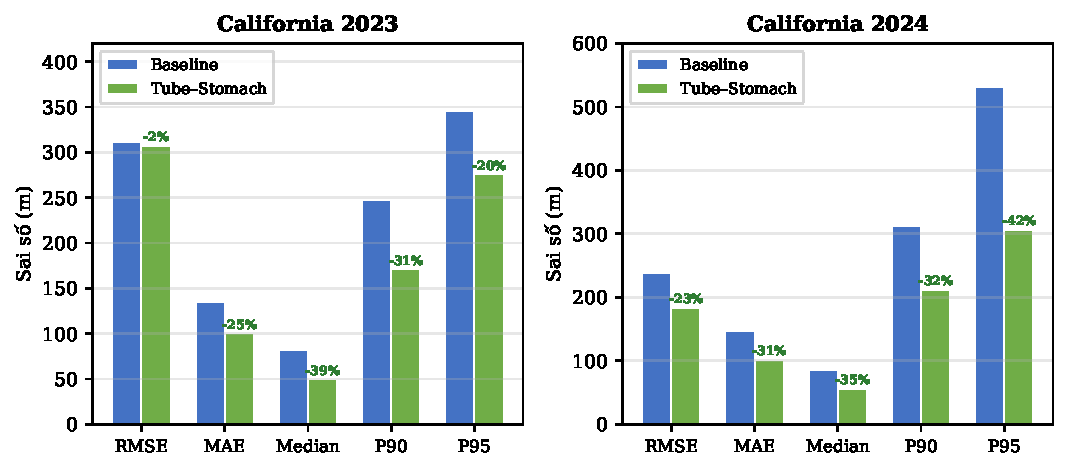
\includegraphics[width=0.88\linewidth]{hinh_1_RMSE_MAE_HIT.pdf}
\caption{So sánh các chỉ số lỗi (RMSE, MAE, Hit@100m) giữa Baseline và Tube--Stomach
trên California 2023 và 2024.}
\label{fig:error-metrics}
\end{figure}

% --- Safety metrics ---
\begin{figure}[H]
\centering
\vspace{-4pt}
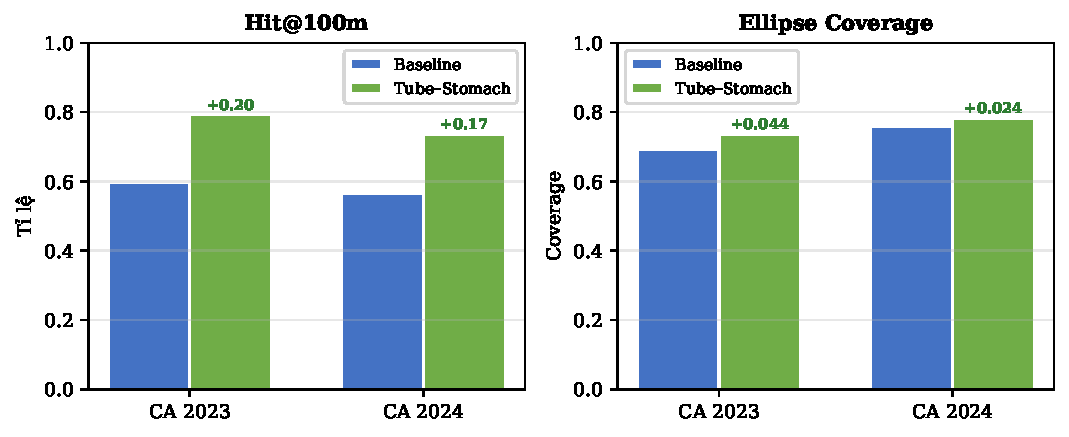
\includegraphics[width=0.88\linewidth]{hinh_2_COV.pdf}
\caption{So sánh chỉ số an toàn--khả dĩ: Ellipse Coverage và Tube Coverage.}
\label{fig:safety-metrics}
\end{figure}

% ============================================================
% Trực quan hóa trên bản đồ
% ============================================================
\subsection{Trực quan hóa trên bản đồ}
Ngoài các thước đo định lượng, chúng tôi tiến hành trực quan hóa dự báo trên bản đồ OSM
để đánh giá tính khả dĩ vật lý trong thực tiễn.
Trường hợp tiêu biểu được lựa chọn là một tàu hàng hải đi dọc theo
luồng vào \textbf{cảng Long Beach / San Pedro} (California),
nơi quỹ đạo chạy song song với đê chắn sóng (breakwater) trước khi rẽ vào cảng.
Đây là kịch bản quan trọng: tàu đổi hướng nhẹ trong hành lang hẹp
gần bờ, baseline dễ tích lũy sai số.

\begin{figure}[H]
  \centering
  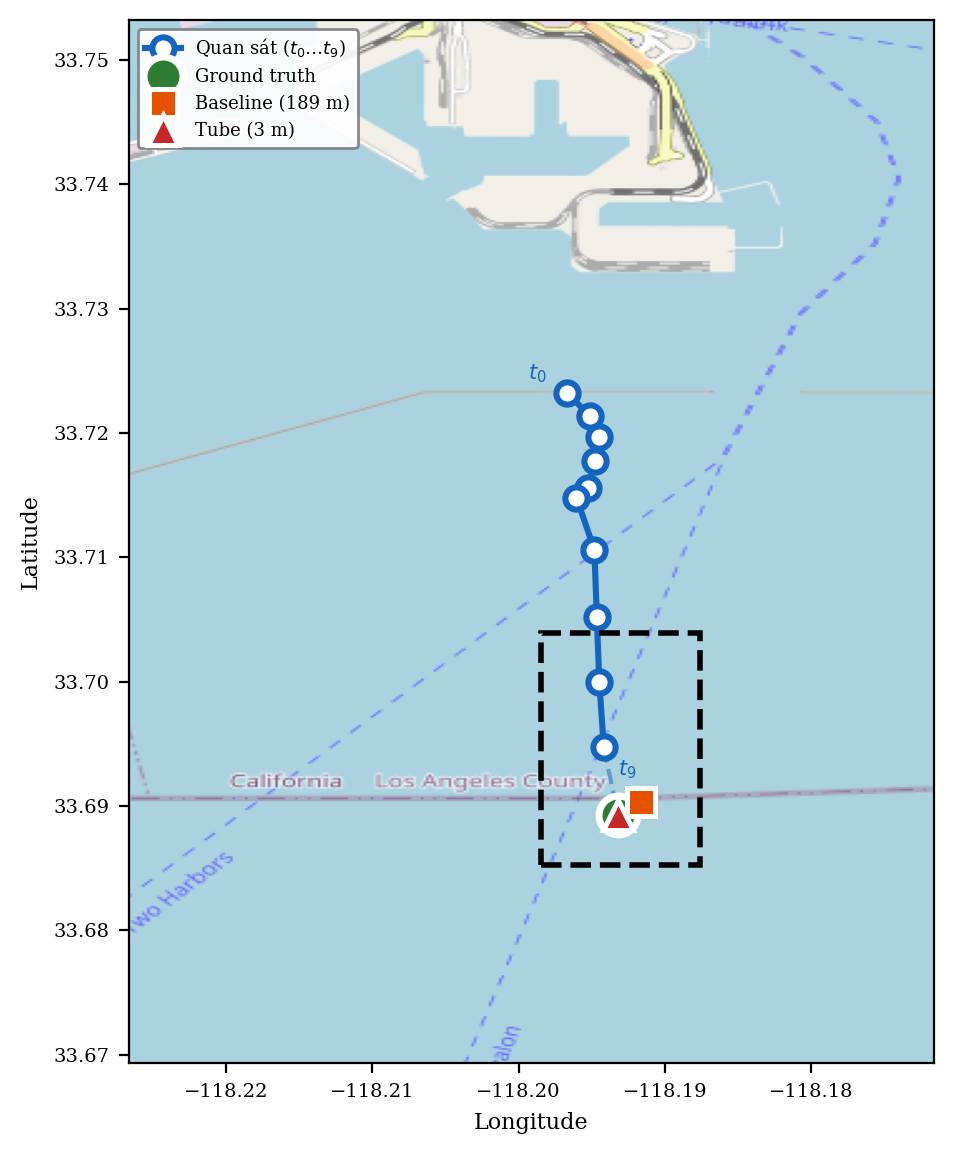
\includegraphics[width=1.0\linewidth]{ban_do_1.png}\\[1ex]
  \subfloat[Baseline --- 189~m]{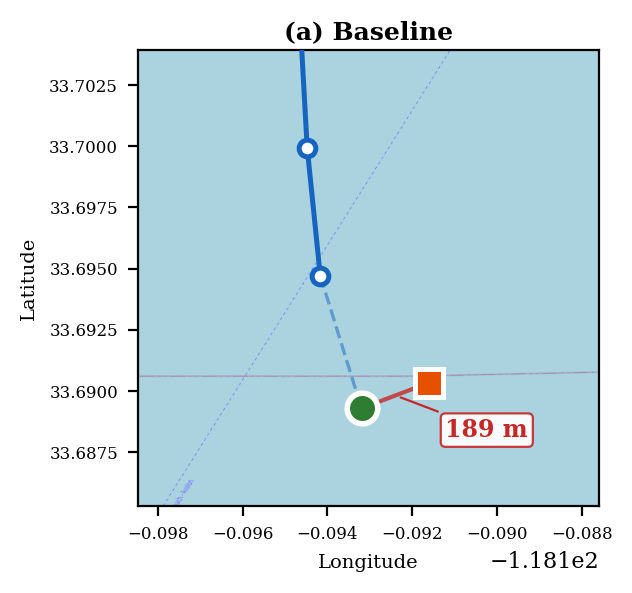
\includegraphics[width=0.48\linewidth]{baseline_ban_do.png}}
  \hfill
  \subfloat[Tube--Stomach --- 3~m]{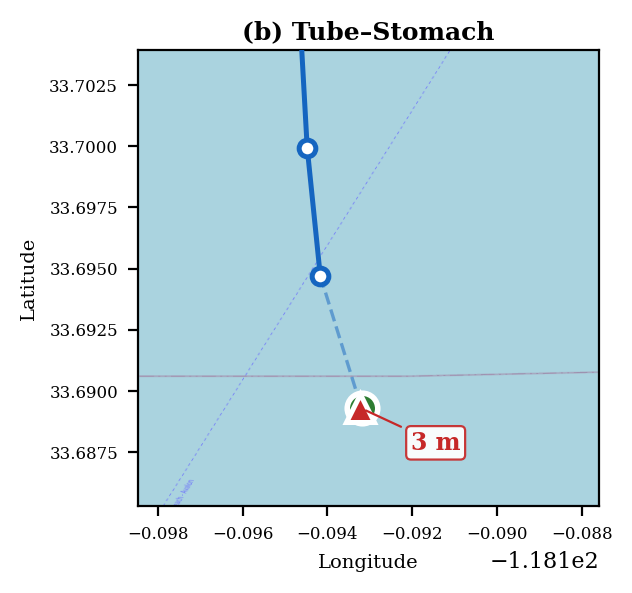
\includegraphics[width=0.48\linewidth]{tube_bando.png}}
  \caption{Trực quan hóa dự báo quỹ đạo gần cảng Long Beach (California).
  (Trên) Toàn bộ 10 bước quan sát ($t_0$--$t_9$) và một bước dự báo ($t_{10}$),
  vùng zoom được đánh dấu tại điểm cuối.
  (Dưới) Zoom-in tại bước $t_{10}$:
  (a) baseline lệch 189~m so với ground truth,
  (b) Tube--Stomach chỉ lệch 3~m, gần như trùng khớp.}
  \label{fig:traj-viz}
\end{figure}

Hình~\ref{fig:traj-viz} trình bày kết quả trực quan:
\begin{itemize}
  \item \textbf{(Trên) Toàn cảnh hành trình:} 10 bước quan sát quá khứ ($t_0 \ldots t_9$)
        và vị trí dự báo ($t_{10}$), trên nền bản đồ thấy rõ cảng Long Beach,
        đê chắn sóng, và khu vực San Pedro. Vùng zoom được đánh dấu
        tại bước cuối để phân tích chi tiết.
  \item \textbf{(a) Baseline (LSTM thuần):} dự báo lệch 189~m so với quỹ đạo thật,
        chệch ra khỏi luồng hàng hải.
        Đây là minh họa trực quan cho việc baseline chỉ dựa thống kê dữ liệu
        mà thiếu đảm bảo vật lý --- khi tàu đổi hướng nhẹ, baseline không bám được.
  \item \textbf{(b) Tube--Stomach:} dự báo gần như trùng khớp với ground truth,
        sai số chỉ 3~m ($-$98\% so với baseline).
        Nhờ ràng buộc hành lang vật lý, mô hình bám sát quỹ đạo thực tế
        ngay cả khi tàu rẽ vào luồng cảng.
\end{itemize}

\medskip
\noindent \textbf{Ý nghĩa.}
Case study này minh họa rõ ràng rằng baseline có thể đạt RMSE trung bình chấp nhận được
nhưng lệch lớn trong từng trường hợp cụ thể (189~m).
Ngược lại, \emph{SphyL--Vessel} với ràng buộc vật lý cho sai số chỉ 3~m ---
gần như trùng khớp quỹ đạo thật.
Điều này vừa cải thiện số liệu định lượng (Hit@100m, Coverage),
vừa củng cố niềm tin khi triển khai trong môi trường hàng hải thực.

% ============================================================
% Phân tích kết quả
% ============================================================
\subsection{Phân tích kết quả}

\textbf{Độ chính xác cơ bản.}
Trên California 2023, Tube--Stomach duy trì RMSE ngang baseline
(311.6~m vs 306.9~m, giảm 1.5\%),
nhưng giảm mạnh MAE ($-$25\%, 134.6~m $\to$ 100.4~m)
và Median ($-$39\%, 81.4~m $\to$ 49.8~m).
Trên California 2024 --- dữ liệu năm khác, kiểm chứng khả năng tổng quát hóa ---
Tube--Stomach phát huy rõ ưu thế:
RMSE giảm 23\% (238.3~m $\to$ 183.4~m),
MAE giảm 31\% (147.7~m $\to$ 101.9~m),
Median giảm 35\% (85.8~m $\to$ 56.1~m).
Điều này chứng minh ràng buộc vật lý mang lại cải thiện nhất quán
trên cả hai năm dữ liệu.

\textbf{Phần đuôi sai số.}
P90/P95 ở California 2023 giảm 70--77~m so với baseline.
Ở California 2024: P90 từ 311.8~m xuống 211.4~m (giảm 32\%);
P95 từ 531.2~m xuống 306.3~m (giảm 42\%).
Điều này cho thấy loss vật lý kiểm soát tốt các tình huống cực trị
như đổi hướng hoặc phanh gấp.

\textbf{Chỉ số an toàn--khả dĩ.}
Hit@100m tăng mạnh: từ 0.596 $\to$ 0.792 ở California 2023
(+33\%, +19.6 điểm phần trăm tuyệt đối)
và từ 0.564 $\to$ 0.736 ở California 2024
(+31\%, +17.2 điểm phần trăm tuyệt đối).
Ellipse Coverage tăng: CA~2023 từ 0.692 $\to$ 0.736;
CA~2024 từ 0.758 $\to$ 0.782.
Outside severity (ellipse) giảm mạnh:
CA~2023 từ 36{,}737 $\to$ 12{,}026 ($-$67\%);
CA~2024 từ 76{,}896 $\to$ 42{,}859 ($-$44\%).

\textbf{Tại sao $\lambda_{\text{tube}}=0.003$ hiệu quả?}
Giá trị $\lambda_{\text{tube\_max}}=0.003$ được chọn qua thử nghiệm:
$\lambda=0.01$ quá lớn khiến MSE bị tube penalty lấn át,
model không hội tụ tối ưu;
$\lambda=0.003$ đủ nhỏ để MSE vẫn là loss chính
nhưng đủ để kéo MAE/Median/Hit@100m vượt trội rõ rệt.
Tube ramp 15 epochs cho phép model ổn định MSE trước khi tube penalty tăng dần,
tránh gradient shock.

\textbf{Chi phí tính toán.}
Tube--Stomach chỉ thêm overhead nhỏ (tích vô hướng, softplus),
thời gian huấn luyện gần như giữ nguyên.
Điều này cho thấy có thể tăng đáng kể tính an toàn mà không cần tới
mô hình nặng như Transformer hay diffusion.

% ============================================================
% Tóm lược mục
% ============================================================
\medskip
\noindent\textbf{Tóm lại Mục 3.}
Mục này đã trình bày:
\begin{itemize}
  \item Tổng quan phương pháp với flow diagram minh họa kiến trúc tổng thể,
        bài toán gốc và tính chất architecture-invariant.
  \item Bộ ký hiệu và khung tọa độ cục bộ (chuyển từ Mục II).
  \item Lộ trình phát triển miền khả đạt: elip cứng $\to$ elip dịch tâm
        $\to$ siêu elip $\to$ Tube--Stomach (chuyển từ Mục II).
  \item Loss lồi--trơn và cơ chế softplus-hinge (chuyển từ Mục II).
  \item Thảo luận biến thể hình học và so sánh ưu/nhược điểm.
  \item Lý do chọn hình học lồi (quán tính tàu, khả vi, tốc độ tính toán).
  \item So sánh chi tiết SphyL--Vessel với PINN và TPK trên nhiều tiêu chí.
  \item Luồng Business Flow (từ thu thập AIS đến đầu ra quỹ đạo dự báo).
  \item Luồng Technical Flow (từ tensor đầu vào đến cập nhật trọng số).
  \item Thiết kế chi tiết mô hình SphyL--Vessel với Tube--Stomach loss
        và tube ramp strategy.
  \item Dữ liệu, tiền xử lý và cấu hình mô hình thực nghiệm.
  \item Thước đo đánh giá và kết quả định lượng trên CA 2023 \& 2024.
  \item Trực quan hóa bản đồ (Long Beach) và phân tích kết quả toàn diện.
\end{itemize}

Kết quả thực nghiệm trên NOAA AIS (California Offshore 2023 và 2024)
đã chứng minh rằng \emph{SphyL--Vessel}:
\begin{itemize}
  \item RMSE giảm 1.5\% (CA~2023) và 23\% (CA~2024);
        MAE giảm 25--31\%; Median giảm 35--39\%.
  \item Hit@100m tăng 17--20 điểm phần trăm tuyệt đối trên cả hai năm.
  \item Ellipse Coverage tăng 2--4 điểm phần trăm;
        Outside severity giảm 44--67\%.
  \item Overhead tính toán nhỏ: chỉ thêm tích vô hướng và softplus,
        không tăng chi phí mô hình.
\end{itemize}

Kết quả này khẳng định rằng chỉ cần một backbone đơn giản (LSTM+attn)
kết hợp loss vật lý convex--smooth,
ta đã có thể đạt dự đoán an toàn và khả dĩ vượt trội.

\end{document}